\bigskip

\thispagestyle{empty}

This is the \textbf{User Manual} for the \texttt{wallcalendar} class.
\textbf{Source documentation} is in \texttt{wallcalendar-code.pdf}. Clone or
download from Github:

\href{https://github.com/profound-labs/wallcalendar/}{https://github.com/profound-labs/wallcalendar/}

The documentclass comes with the following layouts:

\bigskip

\makeatletter
\newlength\exampleWidth
\setlength{\exampleWidth}{45mm}
\makeatother

\begin{extrafullwidth}

\hfill
\begin{minipage}{0.31\linewidth}
\centering

Full page photo, the calendar days\\
overlaid with opacity

\bigskip

\frame{\includegraphics[width=\exampleWidth]{cal-plain-01}}

\end{minipage}%
\begin{minipage}{0.31\linewidth}
\centering

Full page photo, the photo above\\
the calendar days

\bigskip

\frame{\includegraphics[width=\exampleWidth]{cal-plain-02}}

\end{minipage}%
\begin{minipage}{0.31\linewidth}
\centering

Small landscape photo, with a\\
calendar grid

\bigskip

\frame{\includegraphics[width=\exampleWidth]{cal-plain-03}}

\end{minipage}
\hfill\mbox{}

\end{extrafullwidth}

\bigskip

\begin{extrafullwidth}

\hfill
\begin{minipage}[b][40mm][t]{0.31\linewidth}
\centering

Title page

\bigskip

\frame{
\includegraphics[width=\exampleWidth]{./examples/cal-photo-and-notes-titlepage.pdf}}

\end{minipage}%
\begin{minipage}{0.31\linewidth}
\centering

Photo and notes on two pages

\bigskip

\frame{
\includegraphics[width=\exampleWidth]{./examples/cal-photo-and-notes-photo.pdf}}

\smallskip

\frame{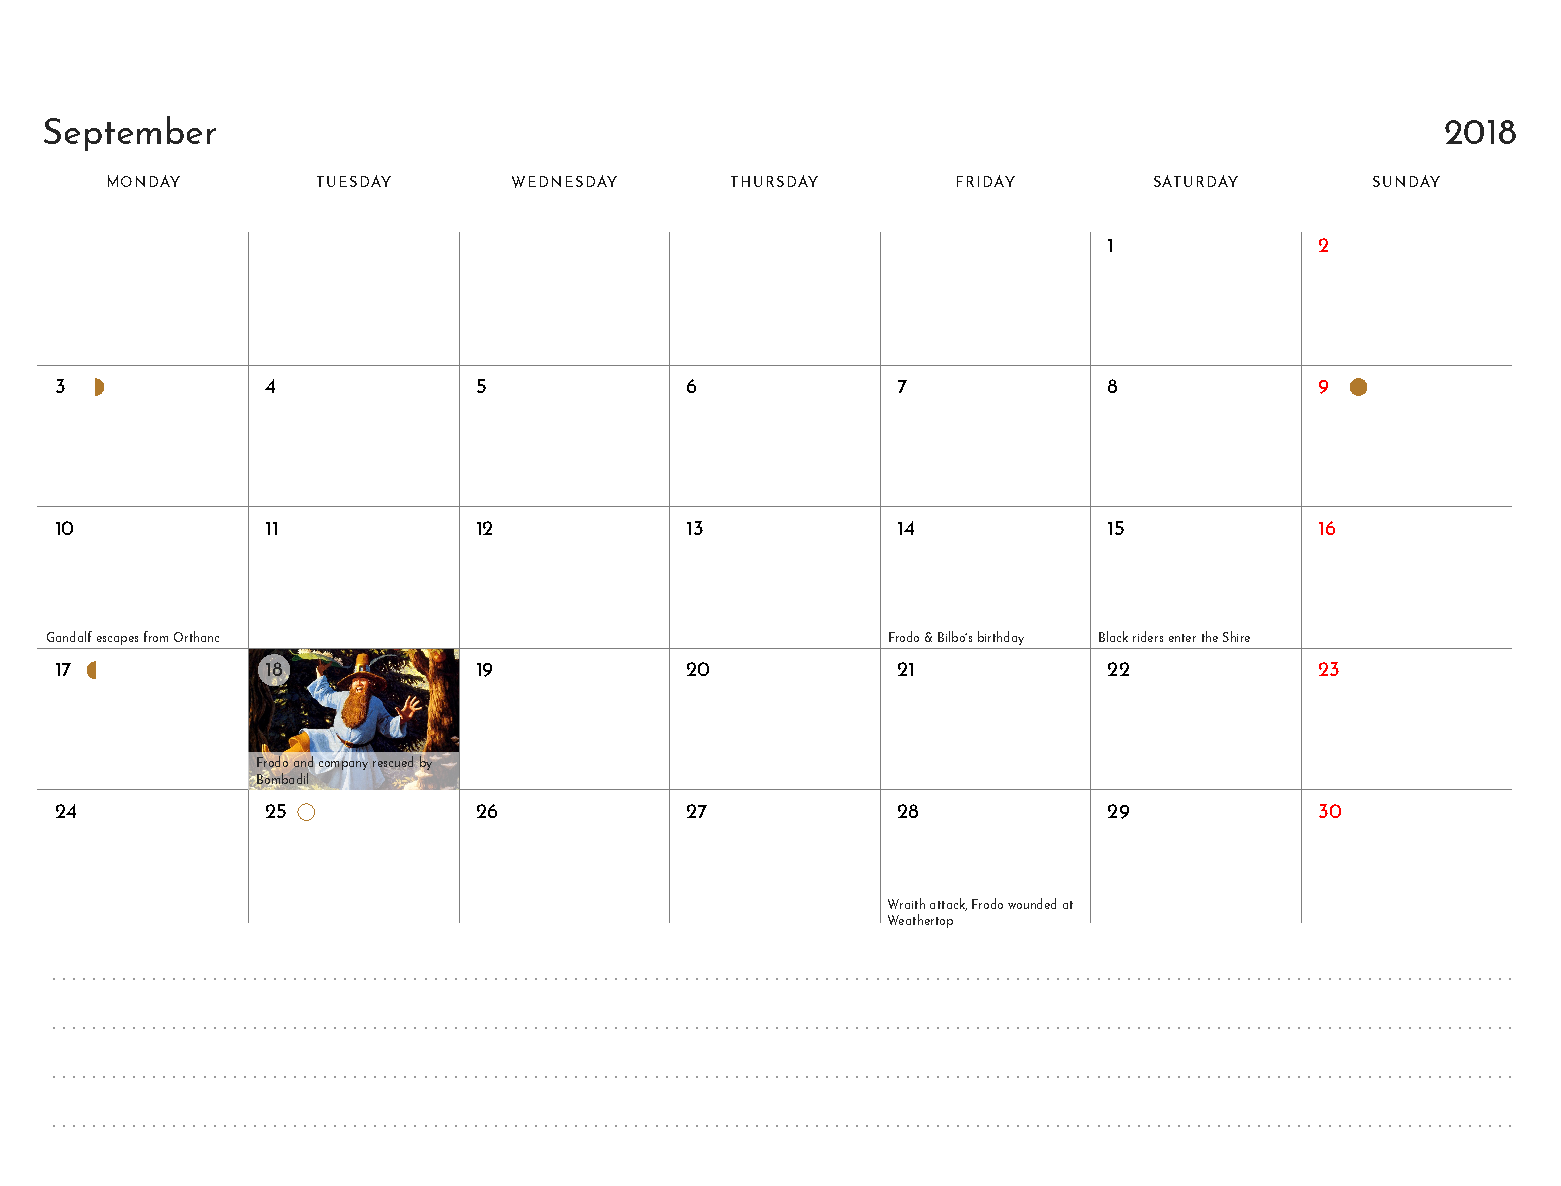
\includegraphics[width=\exampleWidth]{./examples/cal-photo-and-notes-calendar.pdf}}

\end{minipage}%
\begin{minipage}{0.31\linewidth}
\centering

Year planner

\bigskip

\frame{\includegraphics[width=\exampleWidth]{./examples/cal-year-planner.pdf}}

\end{minipage}%
\hfill\mbox{}

\end{extrafullwidth}

\clearpage
\mbox{}\thispagestyle{empty}

\begin{extrafullwidth}

\hfill
\begin{minipage}{0.31\linewidth}
\centering

Load event marks from CSV file

\bigskip

\frame{\includegraphics[width=\exampleWidth]{./examples/cal-marks.pdf}}

\end{minipage}%
\begin{minipage}{0.31\linewidth}
\centering

Thumbnails and captions

\bigskip

\frame{\includegraphics[width=\exampleWidth]{./examples/cal-thumbnails.pdf}}

\end{minipage}
\hfill\mbox{}

\end{extrafullwidth}

\clearpage

\tableofcontents*
\clearpage

